\section{Background}
% Section outline
% Overall summary of section - ~1 sentence per major topic
% ~1 Paragraph for each major topic
\subsection{Introduction}
In this section we will begin with an overview of some existing robotic arms that are currently in industry use in order to gain a high level understanding of what different kinds of arms are out there. Researching the various use cases of existing robotic arms can help us define use cases for our arm. Next, we discuss modular arm technology that is in development in order to have a measure of our progress versus their projects. After examining these arms, we highlight how our project is different from the previously discussed examples and why this is important. Finally, we discuss some of the technology that had to be researched in order to inform our decision on how to design our arm and choose components.

\subsection{Examples of Robot Arms}
There are a few different types of robot arms available on the market today.  Industrial robotic arms, the most common type of arm currently in use are defined as robotic systems used for manufacturing by means of an end effector. Since our arm is relatively small and handles lighter payloads compared to most industrial arms, we will begin with an overview of existing "desktop" industrial arms. Arms that fit this description have a reach of less than one meter. Industrial robot arms typically cost between \$50,000 to \$80,000 new and \$25,000 to \$40,000 used \cite{RobotWorx}. Some manufacturers of these industrial arms include ABB Robotics, Universal Robots, and KUKA Robotics. It's important to note that none of these arms are modular - in fact, they can't be changed at all!

\subsubsection{ABB Robotics}
ABB Robotics makes many small industrial arms. The ABB IRB 120 boasts a 580mm reach, 3kg payload, and 25kg weight. It has 6 degrees of freedom and can be mounted at any angle. The ABB IRB 1200 comes in two varieties, one with a 703mm reach and 7kg payload, and one with a 901mm reach and 5kg payload. Both of these arms have 6 degrees of freedom. The weights are similar at 52kg and 54kg respectively \cite{RobotWorx}.

\begin{figure}[H]
\centering
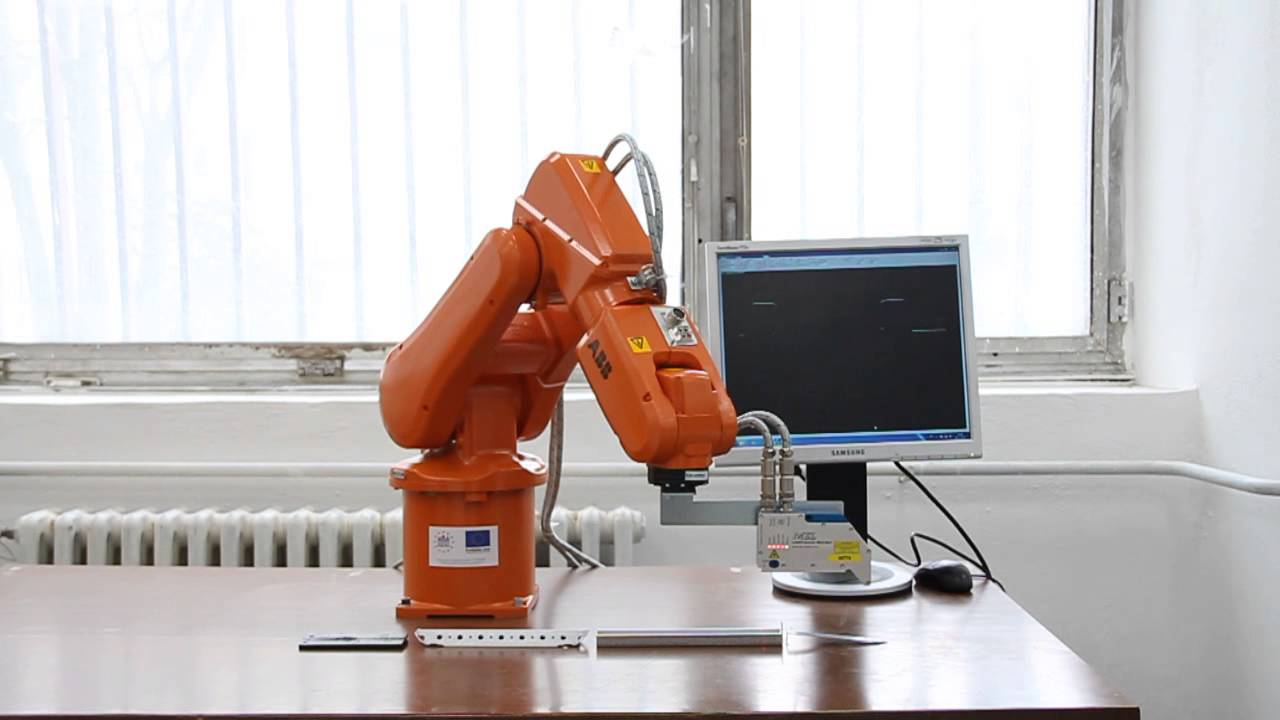
\includegraphics[width=\textwidth]{ABB-irb-120}
\caption{ABB IRB 120 arm \cite{IRB_120}}
\label{fig:abb-irb-120}
\end{figure}

\subsubsection{Universal Robots}
Universal Robots makes two robot arms in this size range. The UR3 is the smaller of the two with a reach of 500mm, payload of 3kg, and 11kg weight. A step up is the UR5 which has a 850mm reach, 5kg payload, and 18.1kg weight. Both of these arms have 6 degrees of freedom. Universal boasts that these arms are easy to implement and re-implement due to compact and lightweight construction, and simple programming interface \cite{RobotWorx}.

\subsubsection{KUKA AG}
KUKA makes two robot arms in this size range. The KR3 R540 has a reach of 541mm, payload of 3kg, and weight of 26kg. It can be mounted on the floor, wall, or ceiling for added utility. The KR 5 sixx R650 is larger with a reach of 650mm, payload of 5kg, and weight of 127kg. It can only be mounted on the floor or ceiling. Both of these arms have 6 degrees of freedom \cite{RobotWorx}.

\subsubsection{Small Industrial Robotic Arm Comparison}
Table \ref{tab:ArmComparison} shows a comparison of all the robotic arms discussed in this section.
\begin{table} [H]
	\centering
	\caption{Comparison of $<$1000mm reach industrial robot arms}
	\label{tab:ArmComparison}
	\begin{tabular}{| l | c | c | c | c |}
		\hline
		\textbf{Name} & \textbf{Reach (mm)} & \textbf{Payload (kg)} & \textbf{Weight (kg)} & \textbf{Axes} \\
		\hline
		IRB120 & 580 & 3 & 25 & 6 \\
		IRB1200-7/0.7 & 703 & 7 & 52 & 6 \\
		IRB1200-5/0.9 & 901 & 5 & 54 & 6 \\
		UR3 & 500 & 3 & 11 & 6 \\
		UR5 & 850 & 5 & 18.1 & 6 \\
		KR3 R540 & 541 & 3 & 26 & 6 \\
		K5 sixx R650 & 650 & 5 & 127 & 6 \\
		\hline
	\end{tabular}
\end{table}

\subsection{Modular Arms}
While there are many industrial arms in production, there are very few modular robotic arms. There is one commercially available robotic arm, the Robolink, made by igus. A few modular robot arms have been developed, including the reconfigurable modular manipulator (RMM), made by TRACLabs \cite{RMM}, and a single joint for the Modular Robotic Arm project MQP at WPI \cite{MRA}.

\subsubsection{igus Robolink} 
Robolink is a modular robotic arm kit produced by the plastics manufacturing company igus.  The kit contains parts to make an arm that is up to 6 Degrees of Freedom (DOF), with belt driven linkages powered by stepper motors that reside in the base of the robot.  Robolink offers 7 individual links, ranging from 1-2 DOF and differing based upon their kind of motion (pivoting, rotating, swiveling).  Each link is made of a lightweight and strong plastic or carbon fiber with cables inlaid in them, resulting in a low cost and weight arm.  The cables used to control these links are made of a high strength synthetic fiber with has a tensile strength of 4,000N.  Separating the actuation of each link from the joint allows the arms to be easily maneuverable with its lightweight and strong joints.  \\
\newline
Purchasers of the kit are able to combine the links in different ways, allowing for a flexible, modular solution to robotic arms. Igus also offers their Robolink software for programming articulated arms that facilitates the programming of individual arms through the use of a simple, intuitive control software. The total cost of a kit to make a 6 DOF arm is \$6000, and buying individual links will cost anywhere from \$370 to \$750 per link. While this price may be low cost compared to other arms such as the ABB robotic arm which can cost up to \$200,000 in total, it is still not low enough for either hobbyists or people interested in learning about robotic arms who are prevented from doing so by the high entry cost. In addition to this, the belt system actuating each link requires the user to thread belts attached to the actuators to each link in order to set up the robot. The long assembly time and intricacy also detracts from the idea of modularity because the time involved in switching configurations can inhibit users from really exploring the different workspaces and combinations this kit can create \cite{igus}.  

\subsubsection{Reconfigurable Modular Manipulator}
The reconfigurable modular manipulator developed by TRACLabs for NASA is a fully modular 7-DOF robot arm. Each joint and end effector have the same connector that provides power and control lines throughout the arm. Internal power and control circuitry take in these lines and convert them into movement. Joints can be swapped out by hand in a matter of seconds. Joints accept position or velocity data from the central communication lines and store physical characteristics about the joints in memory. This robot arm is not commercially available \cite{RMM}.

\subsubsection{Modular Robotic Arm}
This project aimed to close the market gap between inexpensive toy robot arms and expensive professional grade industrial arms. The group aimed to do this by designing a single joint that could be used to assemble a robot arm. Ultimately, a single DOF joint that was heavy, difficult to manufacture, and expensive to produce was designed and constructed. In their future recommendations section, the group stated that the goal of designing a modular robot arm was possible but their design was not the solution \cite{MRA}.

\subsection{Our Robotic Arm System}
Our modular robotic arm aims to offer a completely different use case compared to existing products. The system maintains a low cost while providing a versatile platform for anyone from novice engineers to rapid prototyping professionals. We accomplished this by avoiding expensive proprietary software and subtractive manufacturing; favoring off-the-shelf parts, 3D-printed structures, and freely available/open source software. Providing custom-built software for controlling the arm creates a plug-and-play environment suitable for most any skill level.

\subsection{Technology}
After examining all of these different robot arms accomplished their respective tasks, it was important to go a little more in-depth on how some very crucial components of any robotic arm are chosen and what that means for our project. Some of the most important ideas of an arm are: where does the central processing happen? How can we tell what both the position of and the force on each joint are? It is questions like these that led us to research these key functionalities so that we could make the right choice when we design our arm.  

% \subsection{Communications}
% We looked at several types of communications for the purposes of controlling our robotic arm. These include serial UART, SPI, I2C, and CAN. 
% \subsubsection{Controller Area Network}
% A controller area network (CAN) is a system for sending data reliably between distinct subsystems with reasonably low danger of transmission errors. CAN buses are widely used in the automotive industry to allow various computerized parts of the car to talk to one another.

% Research begins here?
\subsection{Control board}
The control board is meant to be implemented as an independent module that interfaces with a main controller module. Its tasks are to send and receive data from the main controller and control the position of a single motor. As such, the main factors that must be taken into account when designing the control board are methods of measuring joint position and motor torque, as well as communicate with an off-board controller. Motor torque is proportional to motor current. Therefore, the motor torque will be calculated from the measured current through the motor.
\subsubsection{Joint Position Detection}
Angular position sensing must be used to determine the joint angle of the motor. There are several commonly used methods of determining angular position, including potentiometers, optical encoders, and Hall effect sensors \cite{Pot_vs_Sensor,Choose_Sensor_Technology,Choose_Position_Sensor}. A comparison of the different angular sensors can be seen in Table \ref{tbl:Angular_pos_sensors}. \\
\newline
Potentiometers are very commonly used to measure angular position due to their simple implementation and low cost. In addition to being low cost, potentiometers provide high linearity and accuracy \cite{Choose_Position_Sensor}. Although generally robust, these sensors do not lend themselves well to many, rapid adjustments or mechanical vibrations. Both of these significantly reduce the lifespan of the sensor \cite{Pot_vs_Sensor,Choose_Position_Sensor}. The situations potentiometers excel in are those that require an easily adjustable voltage at low to medium adjustment frequencies, such as settings knobs on control panels or analog reference voltages as trim potentiometers \cite{Pot_vs_Sensor}. \\
\newline
Hall Effect sensors are less commonly used, and consist of a bipolar magnet rotating above a Hall effect sensor with the axis of rotation perpendicular to the plane of the sensor. Since there is no contact between the rotation and the sensor, these types of sensors have very long lifespans \cite{Pot_vs_Sensor}. Unfortunately, these sensors do not provide high resolution since they are susceptible to electromagnetic interference and temperature, and also have some hysteresis \cite{Choose_Position_Sensor}. \\
\newline
Optical encoders are another method of measuring angular position. These sensors consist of a beam of light that shines on a slotted disk so that as the disk rotates, the slots break the light beam. These sensors can have very high resolutions and are resistant to shock and vibrations \cite{Choose_Sensor_Technology}. Like magnetic sensors, these sensors have very long lifespans since there is no mechanical connection on the sensor \cite{Pot_vs_Sensor}. Unfortunately, these sensors are susceptible to foreign particles blocking the light beam from sensing the slots and causing incorrect readings. The most common kind of optical encoder, the Quadrature encoder, does not sense absolute position; it can only read relative position, meaning that a quadrature encoder would need to be combined with some other sensor in order for the robot to be able to sense its joint angles correctly. Other encoders called Absolute Optical Encoders do not have trouble reading absolute position, but they are prohibitively expensive. \cite{Choose_Position_Sensor}. \\
\newline
It's worth noting that limit switches can be used to provide information about the location of a joint. Limit switches give a different voltage depending on whether they are pressed or not. When a limit switch is placed at the edge of a particular mechanism's travel range, it becomes possible to determine when the mechanism has reached one of its limits of travel. \\
\newline
Limit switches can be used in conjunction with quadrature encoders (which only provide relative, rather than absolute, position) to create a system which is capable of determining its absolute position. The system would need to go through a homing process at startup whereby the mechanism travels until the limit switch is pressed, at which point the encoders treat their current position as "home".

\begin{table}[H]
	\begin{center}
		\caption{Comparison of different angular position sensors}
		\label{tbl:Angular_pos_sensors}
		\begin{tabular}{ | p{2.4cm} | r | p{1.6cm} | l | l | p{2.5cm} |}
			\hline
			Sensor & Cost & Linearity & Accuracy & Lifespan & Notes
			\\ \hline
			Potentiometer & \$ & Depends on ADC & Moderate & Short & Repeated motion at the same angle can lead to failure
			\\ \hline
			Encoder & \$\$\$ & Very High & Very High & Long & Inexpensive encoders can't sense absolute position
			\\ \hline
			Hall Effect Sensor & \$\$ & High & High & Very Long & Requires special attention to surrounding magnetic fields when mounting
			\\ \hline
		\end{tabular}
	\end{center}
\end{table}

\subsubsection{Current Sensing}
Current sensing can be done in many ways. The most common way is by using a shunt resistor and an amplifier. A variant of this method is to use the resistance inherent in the wires or traces as a shunt resistor. Another common method of current sensing is to use a Hall effect sensor \cite{Current_Sensing}. \\
\newline
Shunt resistors are used in either high side or low side configuration. They are simple to integrate, low cost, and capable of measuring both AC and DC currents. The downsides to this method are relatively large insertion loss that increase exponentially with current, large thermal drift that must be compensated for, as well as large system noise from amplification. There are two main implementations of shunt resistors, high side and low side \cite{Current_Sensing}. \\
\newline
Low side current sensing means that the shunt resistor is placed in the return current path. This method is simpler to implement since the voltage on the shunt resistor is with respect to ground, so it can simply be amplified. Some problems exist with this, however, since the resistor separates the current path from ground. In this configuration, the circuitry used to measure the voltage on the shunt resistor will not report a fault if the system experiences a short circuit \cite{Current_Sensing}. \\
\newline 
High side current sensing means that the shunt resistor is placed on the forward current path. This configuration is able to detect short circuit faults, an advantage to using this configuration over low side current sensing. An additional advantage is that the return current path is directly connected to ground. The downside to high side current sensing is that it requires a differential amplifier since the voltage across the shunt resistor is very close to supply voltage. \cite{Current_Sensing}. \\
\newline
Trace resistance sensing is very similar to using a shunt resistor, but there are some slight differences. Since there isn't a way to control the resistance of a copper trace, the system must be calibrated after being assembled. Another key difference is the amount of amplification needed. Copper traces have very low inherent resistance, so a very large amplification must be used. This large gain imposes a limitation on the maximum measurable bandwidth set by the gain bandwidth product of the amplifier \cite{x}. \\
\newline
Hall effect sensors are commonly used to measure current as well. These sensors can measure current intrusively or non-intrusively, as well as in open loop or closed loop configurations. Non-intrusive devices measure current by wrapping wire around a toroid that focuses the magnetic field on a sensor in a break in the ring of the toroid, or placing the Hall effect sensor on top of the current to be measured. These work fairly well, but are very susceptible to noise from magnetic fields upwards of 10cm away. Methods of shielding these sensors exist, but are complicated and expensive to implement. Intrusive sensors route current through the device and measure the generated magnetic field with a Hall effect device near the current path. Open loop applications take the voltage generated on the Hall effect sensor and condition it to whatever output is needed. Closed loop sensors reroute the sensed current to a secondary coil that is used to generate a proportional current to the measured current. This proportional current is then used as feedback to reduce error \cite{Current_Sensing}. \\
\newline
Insertion loss caused by these sensors is very small. Since these sensors measure current by induction, they can only measure current in a specific frequency band, and high currents at high frequencies can cause these devices to overheat. Most of these frequencies are DC to some upper limit determined by the physical characteristics of the sensor, usually around 100kHz. These sensors cannot be used on their own, since they have an inherent voltage offset, called misalignment voltage, and suffer from high thermal drift. Integrated ICs that compensate for these factors are fairly widespread, allowing for very easy integration \cite{Current_Sensing}.

\subsubsection{Off-Board Communication}
There are many types of communication protocols that could be used to communicate with the main controller. Common protocols include SPI, I$^2$C, RS232, RS485, and CAN. Of these, SPI and I$^2$C are meant mostly for chip to chip communication while RS232, RS485, and CAN are all meant for module to module communication \cite{SerialCompared}. A comparison of these protocols can be seen in Table \ref{tbl:Comm_Compare}. \\
\newline
SPI is a full duplex, synchronous serial link consisting of 3 lines, SCLK, MOSI, MISO, and an additional line for every peripheral, CS. Data rates of up to 10MHz or more are possible due to the elimination of addressing with the CS lines and dedicated clock line \cite{SerialCompared}. Using SPI for controller-to-controller communication presents a problem, however. Since the data transfer rate is controller by the master, the slave could fall behind on processing data. This can be avoided by only transmitting data one direction at a time. Typically, SPI is limited to onboard communications since its signal degrades fairly quickly over distance \cite{CANvSPI}. \\
\newline
I$^2$C is a half duplex, synchronous, multi-master bus consisting of a clock and data line. Data rates of up to 3.4MHz can be reached, and each device has a unique address or multiple addresses to avoid overlap. An interesting aspect of I$^2$C is clock stretching. Clock stretching is when a slave pulls the clock low to stall the master until it has enough time to process information. Typically, I$^2$C is limited to onboard communication since its signal degrades fairly quickly over distance \cite{SerialCompared}. \\
\newline
RS232 is a common full duplex interface that consists of two transmitter/receiver pairs. The protocol limits communication to 1 sender and 1 receiver per line. Data rates of up to 115.2KHz are possible at a range of up to 200ft. Data is typically sent in 8N1 format with 8 data bits, no parity bit, and 1 stop bit or 7E1 format with 7 data bits, even parity bit, and 1 stop bit \cite{SerialCompared}. \\
\newline
RS485 is a full duplex multi-master protocol that consists of up to 32 transceivers on the bus. Data transmission rates of up to 10Mbps and distances of up to 4000ft are possible. Transmission can be reduced to half duplex by removing one transceiver at each node. Data is sent much the same as in RS232 with either 8N1 or 7E1 being common formats \cite{SerialCompared}. \\
\newline
CAN is a half duplex multi-master bus protocol that allows for many nodes to connect and send data on the two transmission lines. Messages are sent with unique addresses that also act as arbitration for bus priority. Packets are fully defined with 11 or 29 bit addresses, 0-8 bytes of data, and some additional control and verification bits \cite{CAN_Guide,CAN_Requirements}. Data rates of up to 1MHz and distances of up to 3000ft are possible. Multiple error checks are implemented at the hardware level since packets are predefined, allowing the controller to load a transmit buffer and let the transceiver send a message or wait until a receive buffer is full before reading the message \cite{CANvSPI}. 
\newline
HID (Human Interface Device) is a communications protocol that defines two entities: the host and the device.  It works by having devices define a data packet and a HID descriptor for the specific device. The host can then receive interrupts from the device during which the pre-defined data packet is transmitted from device to host.  

\begin{table}[H]
	\begin{center}
		\caption{Comparison of off-board communication protocol performance}
		\label{tbl:Comm_Compare}
		\begin{tabular} {| l | l | p{2cm} | p{2.5cm} | p{2.5cm} |}
			\hline
			Protocol & Max Distance & Max Speed & Wires needed & Notes \\ \hline
			SPI & Within circuit board & 10MHz & SCLK, MOSI, MISO, + 1 CS for each node & No addresses needed \\
			\hline
			I$^2$C & Within circuit board & 3.4MHz & 2 & Address included in message \\
			\hline
			RS232 & 200 feet & 115.2KHz & 4 & Can include parity bit \\
			\hline
			RS485 & 4000 feet & 10Mbps & 4 & Can transmit fast or far but not at same time \\
			\hline
			CAN & 3000 feet & 1MHz & 2 & Resilient signal \\
			\hline
		\end{tabular}
	\end{center}
\end{table}


% \begin{figure}[H]
% \centering
% \includegraphics[width=\textwidth]{Detailed_Block_Diagram}
% \caption{Functional block diagram of the system}
% \label{fig:Functional_Block_Diagram}
% \end{figure}